\chapter{関連研究}

\section{XAI}

\subsection{概要}

Wavenet\cite{oord2016wavenet}は
音声波形を時系列データとして自己回帰モデルで学習することによって,人間の声のような自然な音声を生成することができる.
時点$t$における観測値を$x_t$,$\bm{x} = \left\{ x_1, ..., x_T \right\}$を観測値の全体集合とする.このとき,波形の同時確率は条件付き確率の積として
以下のよう表現される.
\begin{equation}
	p(\bm{x}) = \prod_{t=1}^T p(x_t | x_1, ..., x_{t-1})
\end{equation}

つまり,$x_t$は前時点の全てにおけるサンプルに条件づけられる.

\subsection{拡張因果畳み込み}

因果的畳み込み(causal convolutions)がWavenetの最も重要な部分である.
図\ref{fig:ccl}に因果的畳み込み層のスタックを示す.

\begin{figure}[t]
	\centering
	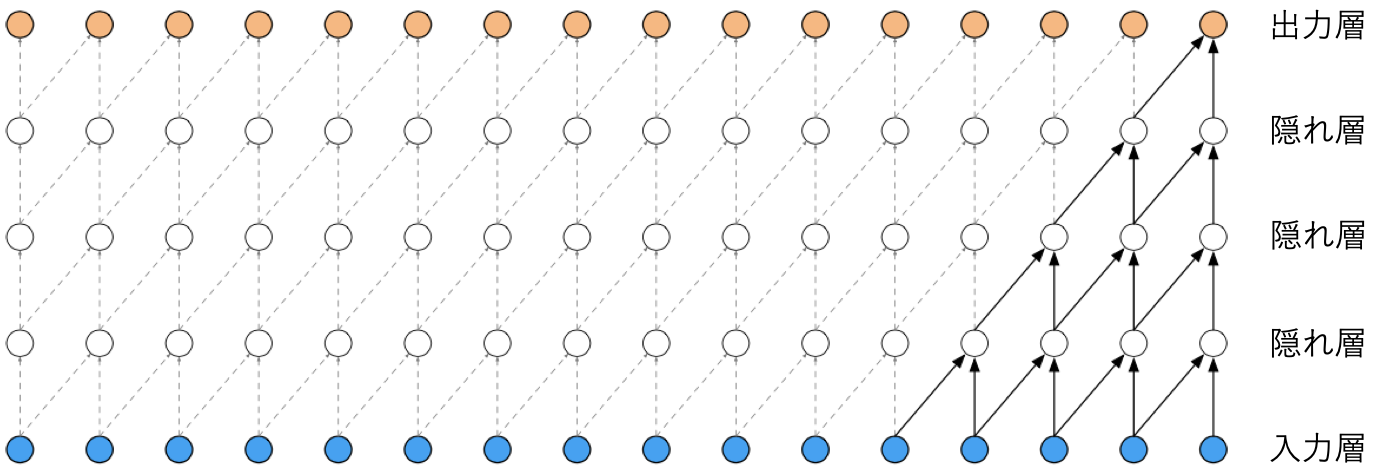
\includegraphics[width=\linewidth]{./figure/ccl.png}
	\caption{因果的畳み込み層}
	\label{fig:ccl}
\end{figure}
